\documentclass[aspectratio=169]{beamer}

% Pacotes essenciais
\usepackage[utf8]{inputenc}
\usepackage[T1]{fontenc}
\usepackage{graphicx}
\usepackage{standalone}
\usepackage{titling}
\usepackage{tikz}
\usetikzlibrary{arrows.meta, positioning, shapes.geometric, calc}

% Carregando o template Cookie
\definecolor{cookieDemoBlue}{HTML}{356AE6}
\usetheme[
  accent=cookieDemoBlue,
  progressbar=foot,
  sectionpage=progressbar,
  numbering=fraction,
  block=fill,
  closing=contact
]{cookie}

% Informações da Apresentação
\title{Open Science}
\subtitle{A Social Duty and its Consequences for Innovation and Reproducibility}
\author{Carlos Henrique Craveiro Aquino Veras}
\cookieemail{carlos.craveiro@usp.br}
\institute{Aerotech Lab - University of São Paulo}
\date{FOSFORUMS 2026}
\cookietagline{FOSFORUMS 2026}
\cookieclosingtitle{That's All Folks!}
\cookieclosingtext{Questions and Discussions are now welcome.}
\cookieclosingqr{https://carloscraveiro.github.io/personal_blog/}
\cookieclosingqrlabel{\url{https://carloscraveiro.github.io/personal_blog/}}

\begin{document}

\maketitle

% Slide de Apresentação Pessoal
\begin{frame}{About Me}
  \begin{columns}[T,onlytextwidth]
    \column{.55\textwidth}
      \cookiekicker{Speaker}
      \vspace{.55em}
      
      \textbf{\theauthor}
      \vspace{.5em}
      
      \begin{itemize}
          \item Computer Engineer from EESC/ICMC - USP.\vspace{.5em}
          \item Master's Student in Mechanical Engineering – Aeronautics at EESC - USP.\vspace{.5em}
          \item A science enthusiast since I can remember and an enthusiast of the FOSS movement since 2021.\vspace{.5em}
          \item I am currently researching the operation of omnidirectional drones at offshore platforms and other intersting topics.
      \end{itemize}

    \column{.40\textwidth}
      \begin{cookiecard}[title=\texttt{printf("Hello World!\textbackslash{}n");}]
        \centering
        \textcolor{cookieMuted}{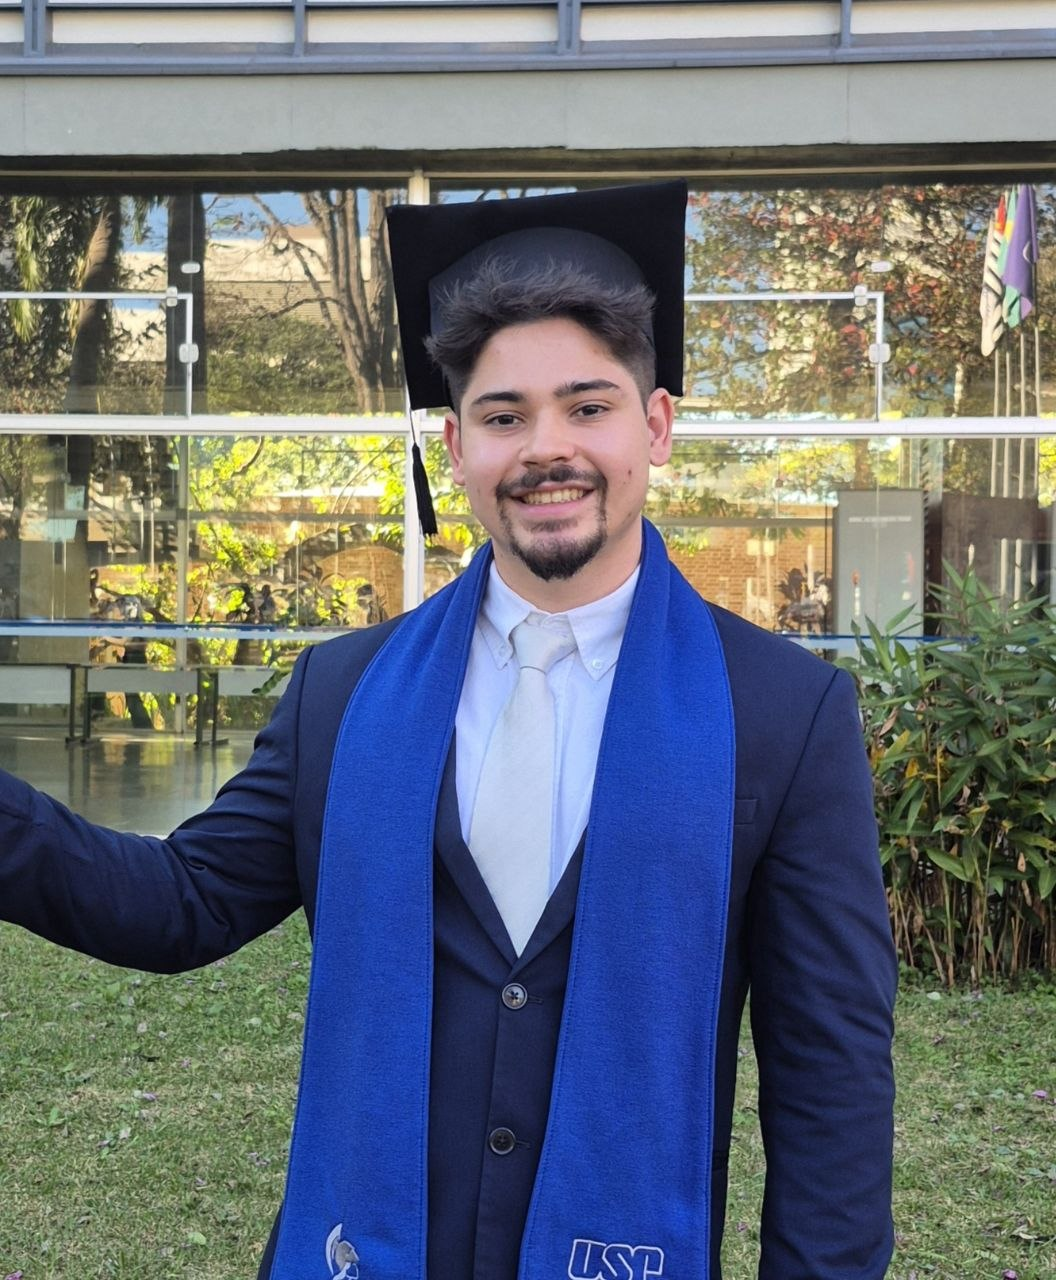
\includegraphics[width=0.9\textwidth]{profile.jpg}}
      \end{cookiecard}
  \end{columns}
\end{frame}

\section{Introducing some concepts}

\begin{frame}{Review of the Scientific Method}
  \begin{columns}[T,onlytextwidth]
    \column{.50\textwidth}
      \begin{itemize}
        \item \textbf{Bibliography research:} Search the state of the art for what has already been done.
        \item \textbf{Peer Review:} Review of the study's merit, methods, and results by external experts.
        \item \textbf{Publication:} Contribute the knowledge gained to the state-of-the-art knowledge base, enabling others to do the same.
      \end{itemize}
      
      \vspace{1em}
      \begin{block}{Question}
        What happens when some points of a study, such as \textbf{methods, data, algorithms}, etc, are \textbf{unclear},  \textbf{missing} or \textbf{not made public}?
      \end{block}

    \column{.45\textwidth}
      \centering
      \vspace{1em}
      \textcolor{cookieMuted}{\resizebox{\textwidth}{!}{\documentclass[tikz,border=15pt]{standalone}
% Pacotes adicionados para garantir que os acentos compilem corretamente
\usepackage[utf8]{inputenc}
\usepackage[T1]{fontenc}
\usetikzlibrary{arrows.meta, positioning, shapes.geometric, calc}

\begin{document}

% =========================================================================
% PALETA DE CORES
% =========================================================================
\definecolor{CorPassoBorda}{HTML}{1A5276}       % Azul Escuro (Borda dos passos normais)
\definecolor{CorPassoFundo}{HTML}{EBF5FB}       % Azul Claro (Fundo dos passos normais)

\definecolor{CorDestaqueBorda}{HTML}{D35400}    % Laranja Escuro (Borda dos passos em destaque)
\definecolor{CorDestaqueFundo}{HTML}{FEF9E7}    % Laranja Claro (Fundo dos passos em destaque)

\definecolor{CorHubBorda}{HTML}{7D3C98}         % Roxo Escuro (Borda do "State of the Art")
\definecolor{CorHubFundo}{HTML}{F5EEF8}         % Roxo Claro (Fundo do "State of the Art")

\definecolor{CorSetaPrincipal}{HTML}{1A5276}    % Azul (Setas do fluxo principal)
\definecolor{CorSetaDestaque}{HTML}{D35400}     % Laranja (Setas de conexão com o Hub)
\definecolor{CorSetaFeedback}{HTML}{7D3C98}     % Roxo (Setas tracejadas de retorno)
% =========================================================================

\begin{tikzpicture}[
    node distance=0.8cm and 2.5cm,
    >=Stealth,
    thick,
    font=\sffamily\large,
    % Configuração dos Estilos
    stepbox/.style={rectangle, draw=CorPassoBorda, fill=CorPassoFundo, minimum width=4.2cm, minimum height=1cm, align=center, rounded corners=3pt},
    emphasis/.style={rectangle, draw=CorDestaqueBorda, fill=CorDestaqueFundo, minimum width=4.2cm, minimum height=1cm, align=center, rounded corners=3pt, font=\sffamily\bfseries\large},
    decisionbox/.style={diamond, aspect=2.2, draw=CorPassoBorda, fill=CorPassoFundo, minimum width=3.5cm, minimum height=1cm, align=center, inner sep=0pt},
    hub/.style={ellipse, draw=CorHubBorda, fill=CorHubFundo, minimum width=4.2cm, minimum height=1.2cm, align=center},
    % Estilos das Linhas/Setas
    mainline/.style={->, line width=1.2pt, draw=CorSetaPrincipal},
    highlightline/.style={->, line width=1.2pt, draw=CorSetaDestaque},
    feedbackline/.style={->, line width=1pt, draw=CorSetaFeedback, dashed}
]

    % --- COLUNA DA ESQUERDA: FLUXO PRINCIPAL ---
    \node[stepbox] (obs) {\textbf{Observation}};
    \node[emphasis, below=of obs] (search) {\textbf{Bibliography Research}};
    
    % (Corrigido) Sem "line breaks" dentro de \textbf{}
    \node[stepbox, below=of search] (hypothesis) {\textbf{Elaborate}\\ \textbf{Hypothesis}};
    \node[stepbox, below=of hypothesis] (experiment) {\textbf{Experiments}};
    \node[stepbox, below=of experiment] (analysis) {\textbf{Analyze Results}};
    
    \node[decisionbox, below=of analysis] (decision) {\textbf{Hypotheses}\\ \textbf{Hold}};
    
    \node[emphasis, below=of decision] (peer) {\textbf{Peer Review}};
    \node[emphasis, below=of peer] (publish) {\textbf{Publication}};

    % --- COLUNA DA DIREITA: CONTEXTO GLOBAL ---
    \node[hub, right=3.5cm of search] (literature) {\textbf{State of the Art}};
    \node[hub, above=1.5cm of literature] (researchers) {\textbf{Other Researchers}};

    % --- CONEXÕES E SETAS ---
    % Fluxo Principal
    \draw[mainline] (obs) -- (search);
    \draw[mainline] (search) -- (hypothesis);
    \draw[mainline] (hypothesis) -- (experiment);
    \draw[mainline] (experiment) -- (analysis);
    \draw[mainline] (analysis) -- (decision);
    
    % Saída SIM do losango
    \draw[mainline] (decision) -- node[right, font=\sffamily\small\bfseries] {\textbf{YES}} (peer);
    \draw[highlightline] (peer) -- (publish);

    % Interações com o "Estado da Arte"
    \draw[highlightline, <->] (search) -- node[above, font=\sffamily\small] {Analyze gaps} (literature);
    
    \draw[highlightline, <->] (researchers) -- node[right, font=\sffamily\small, align=center] {Analyze and\\ contribute} (literature);

    % Ligação Publicação -> Estado da Arte (Faz a curva 90 graus direitinho)
    \draw[highlightline] (publish.east) -| (literature.south);

    % Loop de Feedback (Saída NÃO do losango, contornando pela esquerda)
    \draw[feedbackline] (decision.west) -- ++(-1.8,0) node[above, font=\sffamily\small\bfseries] {\textbf{NO}\phantom{Nooo}} |- (hypothesis.west);

\end{tikzpicture}
\end{document}}}
  \end{columns}
\end{frame}

\begin{frame}[fragile]{Answer: Poor Quality Science}
  \begin{columns}[T,onlytextwidth]
    \column{.48\textwidth}
      \begin{block}{Lack of reproducibility}
        Others have difficulty reproducing or even understanding the published study.
      \end{block}

      \begin{alertblock}{Difficulty extending the work}
        It gets difficult for others to take the study and extend it to other cases, or even use it for \textbf{fair comparison} (in the same conditions) in \textbf{their own studies}.
      \end{alertblock}

    \column{.48\textwidth}
      \begin{alertblock}{Non-falsifiable studies}
        The omission of certain important aspects from the study may render it unfalsifiable, given the \textbf{difficulty of verifying its claims}.
      \end{alertblock}

      \begin{block}{Less citations}
        The \textbf{lack of information} necessary for a study to be better \textbf{understood and replicated} can lead to it being less cited by the community.
      \end{block}
  \end{columns}
\end{frame}

\begin{frame}{Who Funds Scientific Research?}
  \cookiekicker{The Financial Backbone}
  \vspace{.5em}
  
  Historically, science is heavily supported by public resources, the State, or more specifically the \textbf{taxpayer}.\\
  Although the examples are from Brazil, the same situation follows on the rest of the world. 

  \vspace{1em}
  \begin{columns}[T,onlytextwidth]
    \column{.31\textwidth}
      \begin{cookiecard}[title=Public Agencies]
        Direct funding from the State.
        \vspace{.5em}
        
        \cookiebadge{FINEP}
        \cookiebadge{CNPq} \cookiebadge{CAPES}\\
        \cookiebadge{FAPESP}
        \cookiebadge{FAPERJ}
        \cookiebadge{FAPECE}
      \end{cookiecard}

    \column{.31\textwidth}
      \begin{cookiecard}[title=State \& Subsidies]
        State-owned companies and subsidized private R\&D.
        \vspace{.2em}
        
        \cookiebadge{Petrobras (CENPES)}
        \cookiebadge{Embrapa}\\
        \cookiebadge{El Dorado} \cookiebadge{Von Braun}
        
      \end{cookiecard}

    \column{.31\textwidth}
      \begin{cookiecard}[title=Public Universities]
        Research Centers funded by Federal and Regional states government.
        \vspace{.5em}
        
        \cookiebadge{USP} \cookiebadge{Unicamp} \cookiebadge{UNESP} \\
        \cookiebadge{UFRJ} \cookiebadge{UFC} \cookiebadge{UFSCar}
      \end{cookiecard}
  \end{columns}
\end{frame}

\begin{frame}[standout]
  Isn't it fair and ethical that the public have direct and access to the science they fund, especially since it also improves the quality of research?
\end{frame}

\section{Yes! So let's talk about \\ Open Science}

\begin{frame}{What is Open Science?}
  \begin{block}{Definition of \textit{open scientific knowledge} according to UNESCO}
     The unrestricted access to publications, data, metadata, educational resources, software, source code, and hardware made available in the public domain or under open licenses, enabling access, reuse, adaptation, and distribution under specific conditions, free of charge and immediately, to all actors, regardless of their location or individual characteristics.
  \end{block}

  \vspace{1em}
  \begin{columns}[T,onlytextwidth]
    \column{.48\textwidth}
      \cookiekicker{The 3 Core Elements}
      \begin{itemize}
          \item \textbf{Open Access:} Publications \& articles.
          \item \textbf{Open Data:} Raw data, models, specs.
          \item \textbf{Open Source/Processes:} Software, algorithms, and methodologies.
      \end{itemize}

    \column{.48\textwidth}
      \cookiekicker{A Pragmatic Goal}
      \vspace{.5em}
      
      Accelerate scientific, technological, economic, and social progress through active \textbf{collaboration and knowledge reuse}.
  \end{columns}
\end{frame}

\begin{frame}{Core Element 1: Open Access}
  \begin{columns}[T,onlytextwidth]
    \column{.52\textwidth}
      \begin{block}{What does it mean?}
        The \textbf{free}, \textbf{immediate}, and \textbf{unrestricted} online access to scholarly research, allowing anyone to read, download, use, and reuse the work for any lawfull purpose provided the authors receive \textbf{proper credit}.
      \end{block}
      
      \vspace{1em}
      \begin{cookiecard}[title=Traditional vs. Open]
        \centering
        \vspace{0.5em}
        \begin{tikzpicture}[node distance=2mm and 0mm]
          \node[cookie node, draw=cookieAlert, fill=cookieAlert!10, minimum width=3.5cm] (closed) {Paywalled Science};
          \node[cookie node, draw=cookieExample, fill=cookieExample!10, below=of closed, minimum width=3.5cm] (open) {Open Access};
          \draw[cookie arrow, draw=cookieAlert] (closed.east) -- +(1.5,0) node[right, font=\scriptsize, text=cookieInk] {Limited Reach};
          \draw[cookie arrow, draw=cookieExample] (open.east) -- +(1.5,0) node[right, font=\scriptsize, text=cookieInk] {Global Impact};
        \end{tikzpicture}
        \vspace{0.2em}
      \end{cookiecard}

    \column{.43\textwidth}
      \cookiekicker{Open Access History}
      \vspace{.5em}
      
      More than 40 years of history, but four key events were:
      \vspace{.5em}
      
      \begin{itemize}
        \item \textbf{Santa Fe (1999):} Interoperability and metadata protocol (OAI-PMH).
        \item \textbf{Budapest (2002):} Coined and defined "Open Access".
        \item \textbf{Bethesda (2003):} Defined open publishing and user rights.
        \item \textbf{Berlin (2003):} Committed global research institutions.
      \end{itemize}
  \end{columns}
\end{frame}

\begin{frame}{Core Element 2: Open Data}
  \cookiekicker{Beyond just publishing data}
  \vspace{.5em}
  
  Simply ''dumping'' data online is not enough. For data to be truly open and useful to the community, it must follow the \textbf{FAIR} principles:
  \vspace{-.5em}
  \begin{columns}[T,onlytextwidth]
    \column{.48\textwidth}
      \begin{cookiecard}[title=F - Findable]
        Data must have rich metadata and a unique, persistent identifier (like a DOI) so both humans and computers can easily find it.
      \end{cookiecard}
      
      \vspace{0.1em}
      \begin{cookiecard}[title=A - Accessible]
        Once found, users need to know how to access it, usually through standard, open, and universally implementable protocols.
      \end{cookiecard}

    \column{.48\textwidth}
      \begin{cookiecard}[title=I - Interoperable]
        Data should be formatted in ways that allow it to be integrated with other datasets and analyzed by different software.
      \end{cookiecard}
      
      \vspace{0.1em}
      \begin{cookiecard}[title=R - Reusable]
        Data must be well-documented, clear in its context, and released with a highly accessible data usage license.
      \end{cookiecard}
  \end{columns}
\end{frame}

\begin{frame}{Core Element 3: Open Source, Hardware \& Processes}
  \begin{columns}[T,onlytextwidth]
    \column{.48\textwidth}
      \cookiekicker{The Problem with ''Black Boxes''}
      \vspace{.5em}
      
      \begin{alertblock}{Proprietary Tools Harm Science}
        Closed software (e.g., MATLAB toolboxes) or other proprietary solutions create severe barriers:
        \vspace{0.5em}
        \begin{itemize}
          \item \textbf{Access Barriers:} Replicating results requires buying expensive licenses or exact equipment, locking out researchers or pushing them toward piracy.
          \item \textbf{Hidden Mechanics:} If a method fails on a different setup, you cannot investigate the root cause without access to the source code or schematics.
        \end{itemize}
      \end{alertblock}

    \column{.48\textwidth}
      \cookiekicker{The Open Solution}
      \vspace{.5em}
      
      \begin{block}{FOSS \& Open Hardware}
        Sharing actual code, algorithms, and hardware blueprints ensures:
        \vspace{0.5em}
        \begin{itemize}
          \item \textbf{Deep Investigation:} Full transparency to debug and understand exactly \textit{how} and \textit{why} a technique works.
          \item \textbf{Ease of Customization:} Freedom to edit intrinsic features to adapt the tool to your specific needs.
          \item \textbf{Community Ecosystem:} Contributions are easily assimilated, enriching available tools and fostering true collaboration.
        \end{itemize}
      \end{block}
  \end{columns}
\end{frame}

\section{Benefits of Open Science}

\begin{frame}{For Scienc and Researchers}
  \begin{columns}[T,onlytextwidth]
    \column{.48\textwidth}
      \cookiekicker{For the Scientific Field}
      \vspace{.5em}
      
      \begin{itemize}
        \item \textbf{Robustness:} Enables independent validation and true reproducibility.
        \item \textbf{Innovation:} Fosters multidisciplinary collaboration and the creation of new tools.
        \item \textbf{Democratization:} Reduces global inequalities by lowering access barriers to knowledge.
        \item \textbf{Preservation:} Guarantees long-term data integrity in public repositories.
      \end{itemize}

    \column{.48\textwidth}
      \cookiekicker{For the Researcher}
      \vspace{.5em}
      
      \begin{itemize}
        \item \textbf{Visibility:} Expands research networks and boosts citations.
        \item \textbf{Resource Economy:} Reusing existing data saves time and precious funding.
        \vspace{0.3em}
        
        \cookiebadge{Human Genome Project} \cookiebadge{Data Amazon (USP)}
        \vspace{0.5em}
        
        \item \textbf{New Analyses:} Crossing different datasets generates unique insights.
        \item \textbf{Integrity:} Enhances personal accountability and academic reputation.
      \end{itemize}
  \end{columns}
\end{frame}

\begin{frame}{For the Society}
  \begin{columns}[T,onlytextwidth]
    \column{.45\textwidth}
      \begin{cookiecard}[title=Access to Knowledge]
        Open access to articles and data directly benefits \textbf{education}, \textbf{innovation}, and \textbf{social development}.
      \end{cookiecard}
      
      \vspace{1em}
      \begin{cookiecard}[title=Institutional Transparency]
        Increases the \textbf{visibility of universities} and research centers, helps to \textbf{demonstrates their social importance} and impact.
      \end{cookiecard}

    \column{.50\textwidth}
      \vspace{1em}
      \cookiekicker{Public Engagement}
      \vspace{.5em}
      
      It fosters an understanding of \textbf{how science works}, its methods and methodologies, \textbf{empowering scientific communication} and dissemination, hence its importance.
      
      \vspace{1em}
      \centering
      \begin{tikzpicture}
        \node[cookie accent node, minimum width=3cm, minimum height=1cm, font=\bfseries] (soc) {Society};
        \node[cookie node, below left=0.5cm and -0.5cm of soc, minimum width=2.2cm, font=\small] (edu) {Education};
        \node[cookie node, below right=0.5cm and -0.5cm of soc, minimum width=2.2cm, font=\small] (inv) {Innovation};
        \draw[cookie arrow] (soc) -- (edu);
        \draw[cookie arrow] (soc) -- (inv);
      \end{tikzpicture}
  \end{columns}
\end{frame}

\begin{frame}{A Matter of Comprehension and Democracy}
  \begin{columns}[T,onlytextwidth]
    \column{.35\textwidth}
      % Espaço para foto do Carl Sagan ou ilustração do livro
      \centering
      \textcolor{cookieMuted}{\begin{figure}
          \centering
          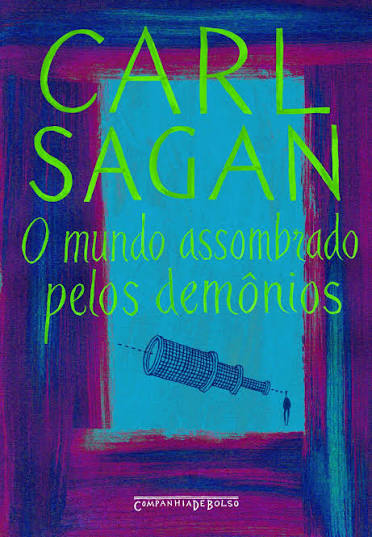
\includegraphics[width=0.8\linewidth]{demon_haunted_world.jpeg}
          \caption{The Demon-Haunted World (Brazilian edition cover).}
          \label{fig:carlsagan}
      \end{figure}}
      
    \column{.60\textwidth}
      Direct access \textbf{fosters public respect} while \textbf{deepening the understanding of scientific methods}, tools, and limitations. Crucial for informed citizenship in a democratic society.
      
      \vspace{0.5em}
      \begin{cookiequote}[Carl Sagan]
      \normalsize
        We've arranged a global civilization in which most crucial elements profoundly depend on science and technology. We have also arranged things so that nobody understands science and technology. This is a prescription for disaster. We might get away with it for a while, but sooner or later this combustible mixture of ignorance and power is going to blow up in our faces.
      \end{cookiequote}
      \hfill \textit{(The Demon-Haunted World)}
  \end{columns}
\end{frame}

\section{Guides for practicing\\Open Science}

\begin{frame}{How to Do Open Science: Publishing \& Materials}
  \begin{columns}[T,onlytextwidth]
    \column{.48\textwidth}
      \cookiekicker{1. Open Access Publishing}
      \vspace{.5em}
      
      Publish your work in \textbf{Open Access (OA) journals}.
      \begin{itemize}
        \item If full OA is not possible, utilize \textbf{pre-print servers} (like arXiv) to share early versions. 
        \item \textit{Note: Pre-prints are not peer-reviewed yet, but ensure immediate public access.}
      \end{itemize}

            \begin{figure}
            \centering
            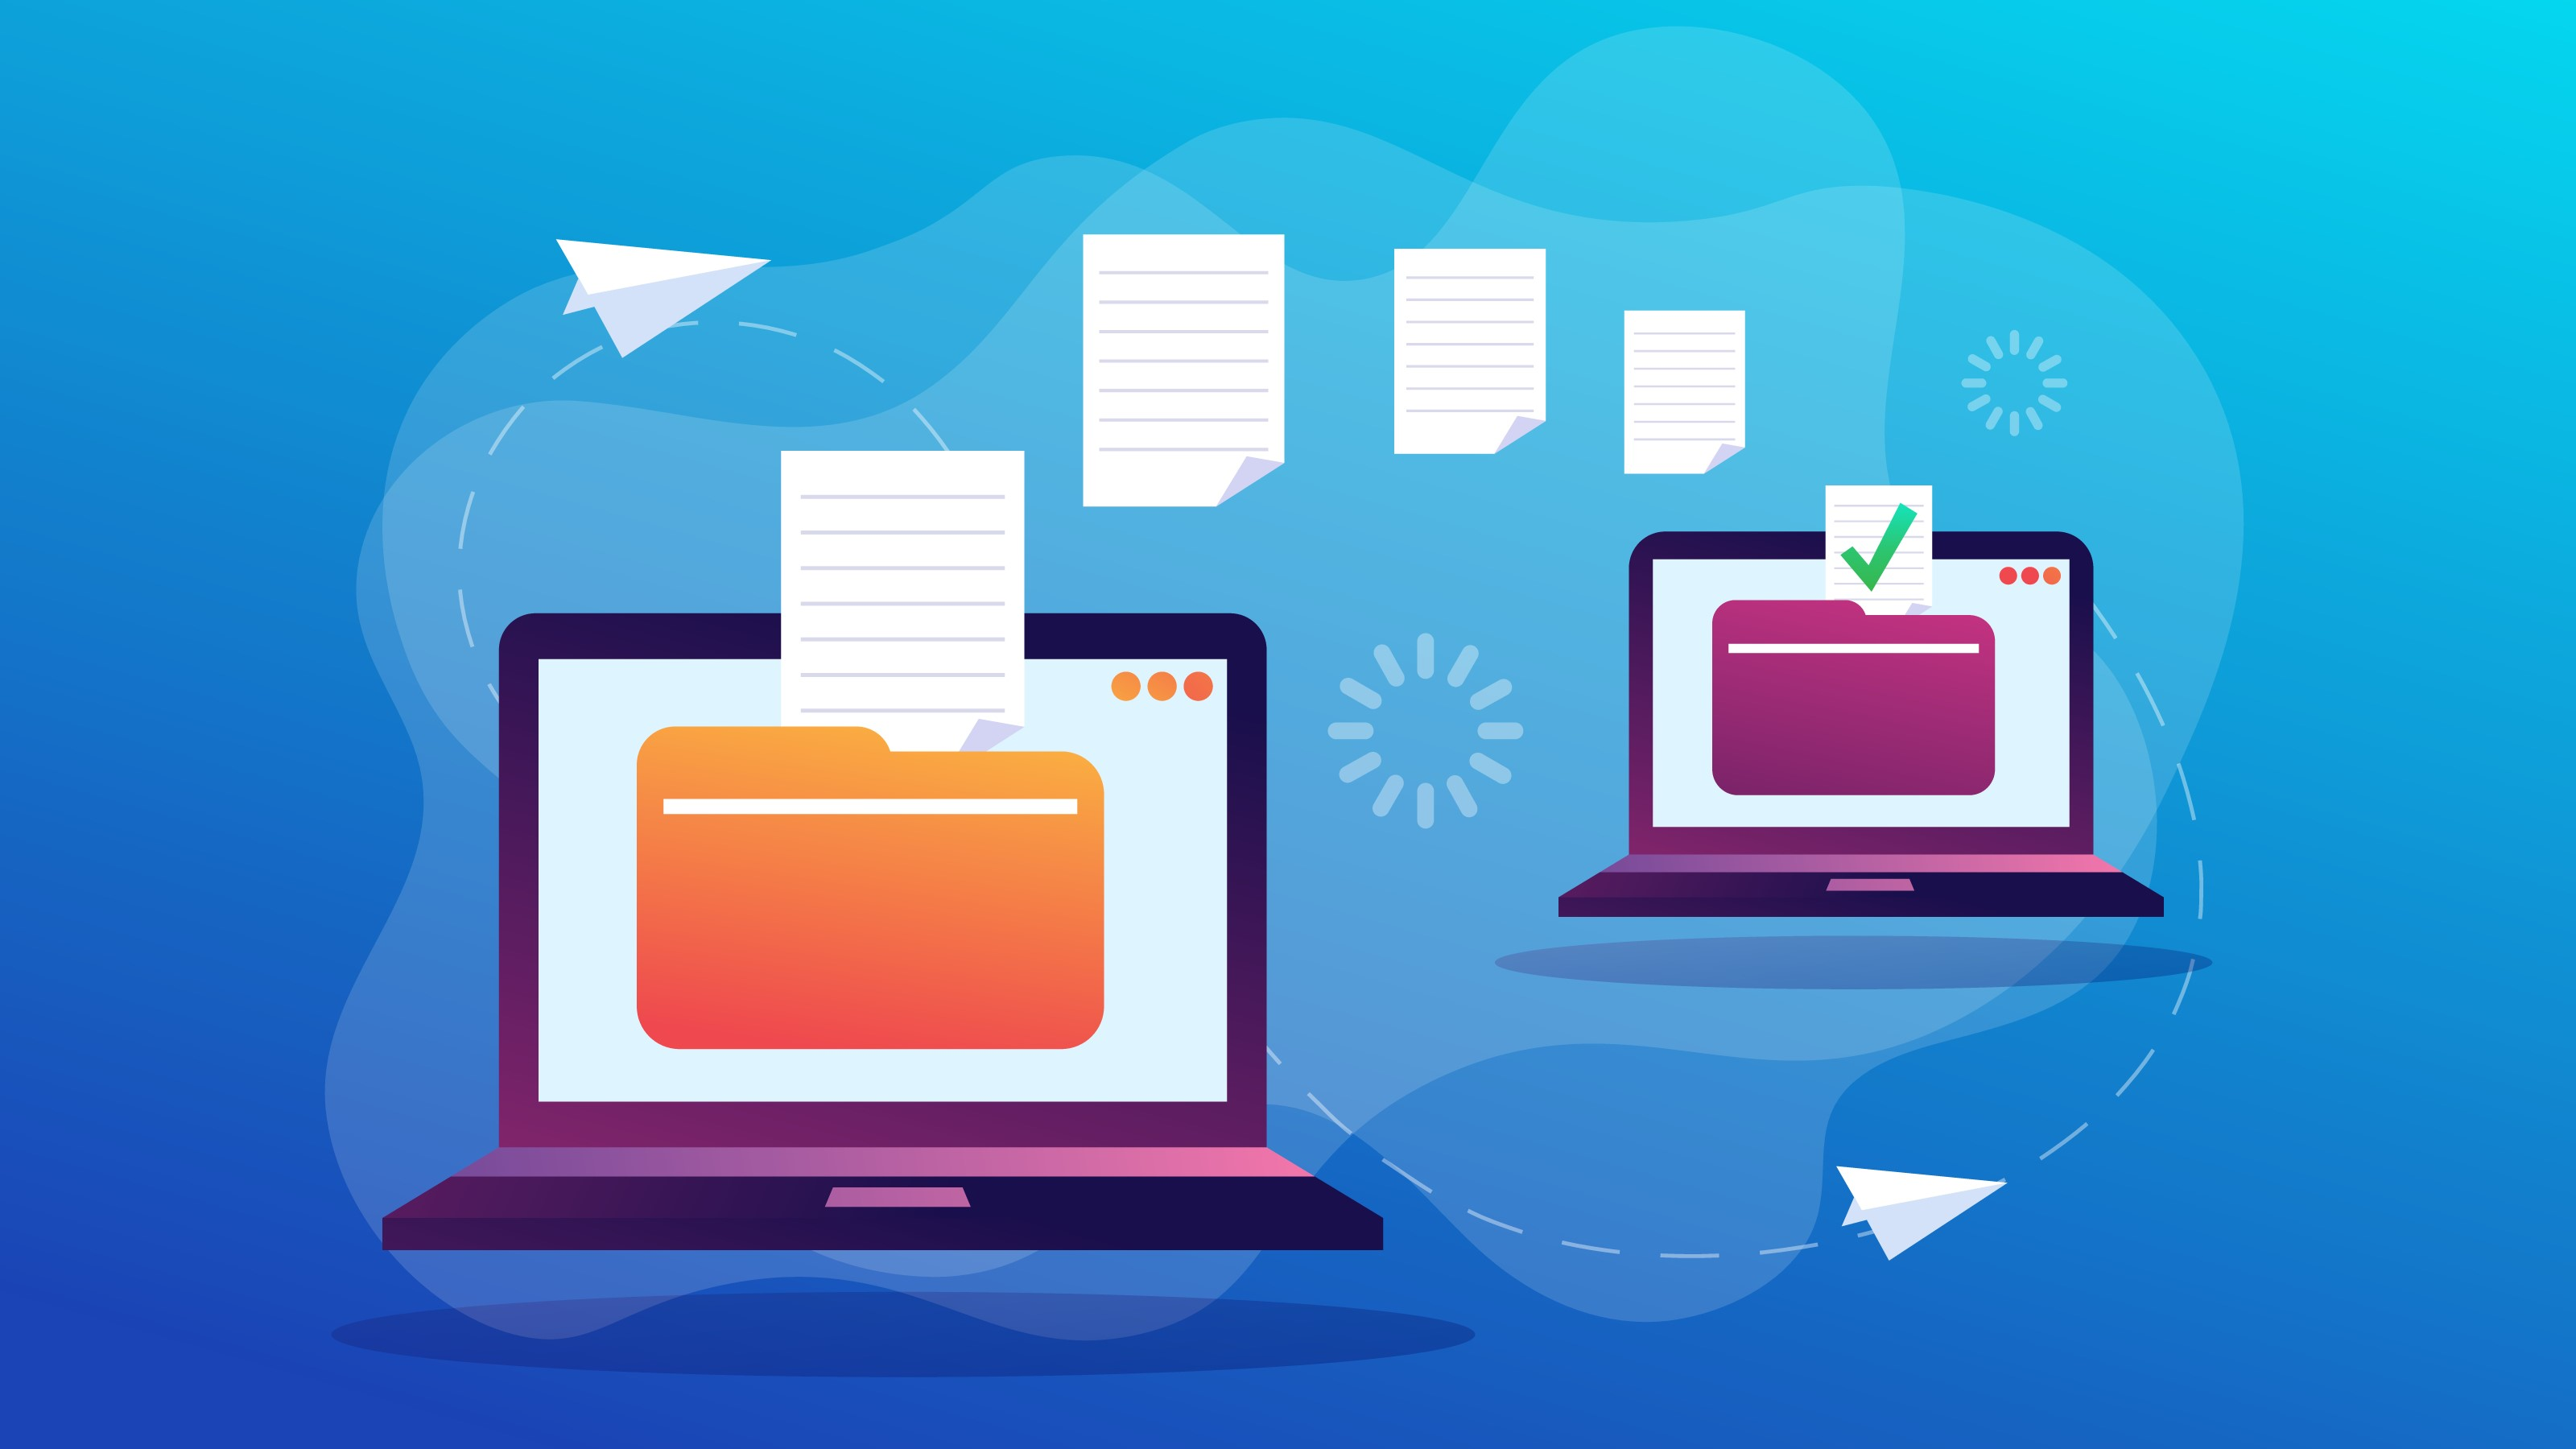
\includegraphics[width=0.8\linewidth]{sharing_data.jpg}
        \end{figure}

    \column{.48\textwidth}
      \cookiekicker{2. Share Auxiliary Materials}
      \vspace{.5em}
      
      Don't hide the "messy" but crucial details that don't fit in the main paper. Share:
      \begin{itemize}
        \item Complete mathematical deductions.
        \item In-depth descriptions of methods and procedures.
        \item Extended datasets and raw outputs.
      \end{itemize}
      \vspace{0.5em}
      \begin{cookiecard}[title=The Main Point]
        Make your work easy to understand, even for professionals from other fields, and also easy to reproduce.
      \end{cookiecard}
  \end{columns}
\end{frame}

\begin{frame}{How to Do Open Science: Tools \& Data}
  \begin{columns}[T,onlytextwidth]
    \column{.48\textwidth}
      \cookiekicker{3. Open Tools \& Licensing}
      \vspace{.5em}
      
      \textbf{Prioritize FOSS solutions} for your research. If you develop new ones, release them openly!
      \begin{itemize}
        \item \textbf{Least Alternative for Hardware:} If you really cannot make it open, \textbf{at least patent it}. Patents require a detailed description that inherently allows for future reproduction of the idea.
      \end{itemize}
        \begin{figure}
            \centering
            
\includegraphics[width=0.75\linewidth]{FOSS.png}
        \end{figure}
    \column{.48\textwidth}
      \cookiekicker{4. Open Data (FAIR)}
      \vspace{.5em}
      
      Publish your datasets following the \textbf{FAIR} principles.
      
      \vspace{1em}
      \begin{alertblock}{Watch out for LGPD / GDPR!}
        \textbf{Anonymization is key.} Be careful when opening data involving human subjects. Always follow:
        \begin{itemize}
          \item LGPD (General Data Protection Law).
          \item Ethical and bioethical guidelines.
          \item Common sense to protect privacy.
        \end{itemize}
      \end{alertblock}
  \end{columns}
\end{frame}

\begin{frame}{Open Data \& Privacy: The LGPD}
  \cookiekicker{Brazilian General Data Protection Law (Law 13,709/2018)}
  \begin{columns}[T,onlytextwidth]
    \column{.48\textwidth}
      \begin{block}{For Academics: Compliance Basics}
        \begin{itemize}
          \item \textbf{Informed Consent (Art. 8):} Data collection requires clear, unambiguous consent for specific research purposes.
          \item \textbf{Anonymized Data (Art. 12):} Truly anonymized data is \textbf{not} considered personal data under the law. The legal foundation that makes sharing Open Data possible.
          \item \textbf{Security (Art. 46):} Researchers must adopt strict technical measures to protect raw data from leaks before it is anonymized and published.
        \end{itemize}
      \end{block}

    \column{.48\textwidth}
      \begin{exampleblock}{For the Public: Peace of Mind}
        Consenting \textbf{does not} mean giving up your privacy.
        
        \vspace{0.5em}
        
        The Law states that shared data must consist strictly of \textbf{scientific variables}, ensuring the candidate's privacy. All names, IDs, and personal traces are stripped away before publication to guarantee that data cannot be used for discriminatory purposes.
      \end{exampleblock}
      \vspace{-0.5em}
      \begin{figure}
          \centering
          
\includegraphics[width=0.7\linewidth]{LGPD_1.png}
      \end{figure}
  \end{columns}
\end{frame}

\section{The Challenges of Open Science}

\begin{frame}{The Hard Truth: Open Science Takes Work}
  \begin{alertblock}{The Main Issue}
    Doing Open Science demands more effort, time, and resources than traditional "closed" science, simply because ensuring \textbf{true reproducibility is hard}, and sometimes \textbf{expensive}.
  \end{alertblock}

  \begin{columns}[T,onlytextwidth]
    \column{.48\textwidth}
      \cookiekicker{Financial and Time Costs}
      \vspace{.5em}
      \begin{itemize}
        \item Article Processing Charges (APCs) for \textbf{Open Access journals} are often very \textbf{expensive}.
        \item Costs associated with \textbf{long-term data storage} and repository maintenance.
        \item Cost associated with ensuring \textbf{readability}, \textbf{scalability}, and \textbf{documentation}, as well as the time spent contributing to projects and managing a community.
      \end{itemize}

    \column{.48\textwidth}
      \cookiekicker{Technical \& Human Resources}
      \vspace{.5em}
      \begin{itemize}
        \item Requires specific knowledge in \textbf{data stewardship}.
        \item Writing and contributing to maintainable/open-source software/hardware projects demands specific skills and knowledge.
        \item Needs specialized personnel for \textbf{documentation}, \textbf{project} and \textbf{community management}.
      \end{itemize}
  \end{columns}
\end{frame}

\begin{frame}{Alleviating the Finantial Costs: Institutional Support}
  \cookiekicker{Good news for Brazilian Researchers}
  \vspace{.5em}
  
  Recent agreements by CAPES are helping to waive or reduce Article Processing Charges (APCs) for Brazilian authors in major publishers.
  \centering
  \begin{cookiecard}[title=News Highlight from FAPESP Magazine - Feb 2026 - CC-BY-NC-ND. By: Sarah Schmidt]
    \textcolor{cookieMuted}{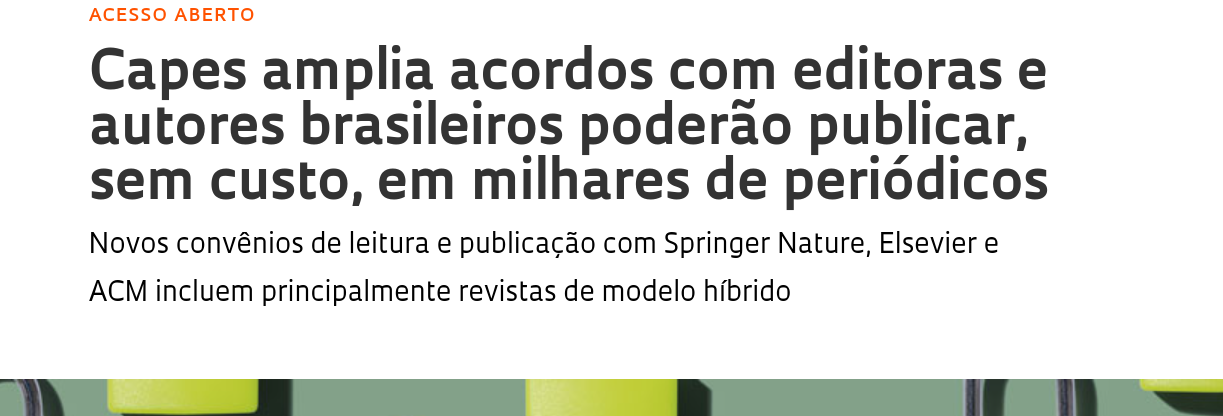
\includegraphics[width=\linewidth]{Screenshot-2026-08-28_08-42-30.png}}
  \end{cookiecard}
\end{frame}

\begin{frame}{Institutional Platforms for Data Long-Term Storage}
     \cookiekicker{Other form of institutional support}
  \vspace{.5em}
  
  Some big public research institutions host their own open data "repos", such as Unicamp with its Digital Educational Repository (REDU), thus absorbing the financial cost to host the data for long periods of time. 
  \centering
  \begin{cookiecard}[title=Unicamp's Open Data Repository (REDU)]
    \textcolor{cookieMuted}{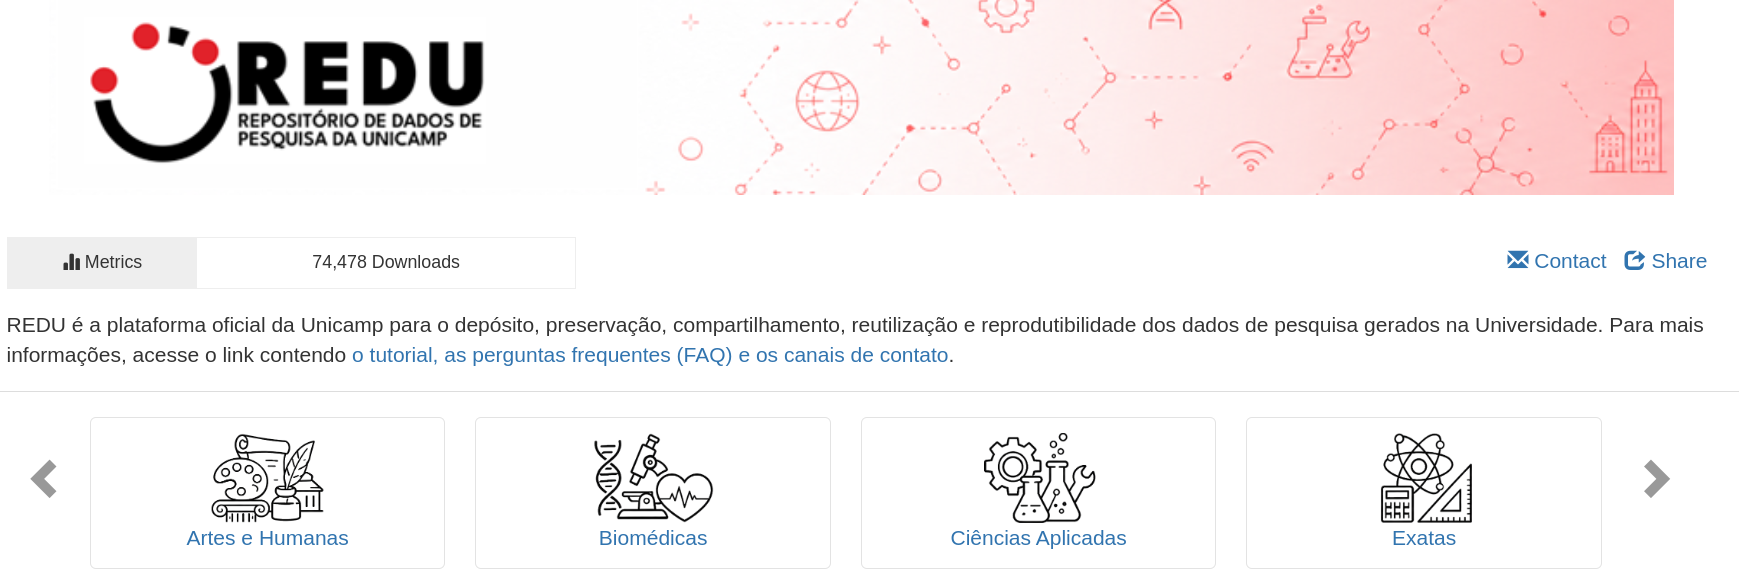
\includegraphics[width=\linewidth]{Screenshot-2026-08-28_11-58-29.png}}
  \end{cookiecard}
\end{frame}

\begin{frame}{The Role of the Research Software Engineer (RSE)}
  \begin{columns}[T,onlytextwidth]
    \column{.48\textwidth}
      \cookiekicker{Who is the RSE?}
      \vspace{.5em}
      
      A professional who combines a deep understanding of \textbf{research} with reasonable \textbf{software engineering} skills and knowledge.
      
      \vspace{1em}
      \begin{exampleblock}{Between Two Worlds}
        As we saw, technical challenges (data stewardship, code documentation, community building) are major barriers to Open Science. So, we need someone who \textbf{understands both worlds} to solve this problem.

      \end{exampleblock}

    \column{.48\textwidth}
      \cookiekicker{Why are they essential?}
      \vspace{.5em}
      
      The RSE directly tackles the technical challenges of Open Science by:
      \begin{itemize}
        \item Building robust, reusable, and open research software.
        \item Ensuring code and data follow FAIR principles.
        \item Writing high-quality documentation that allows the community to actually use the tools.
        \item Taking the burden of "software maintenance" off the shoulders of traditional scientists.
      \end{itemize}
  \end{columns}
\end{frame}

\begin{frame}{One case of Personal Experience}
     \cookiekicker{From a lab where I did a research internship abroad}
  \vspace{.5em}
  
  The principal investigator is interested in making the ecosystem open, but although the code is available, the documentation is not yet good enough for an outsider to reproduce and contribute to the environment without full assistance from internal staff. \textbf{Lacks a lot of crucial information}.
  \vspace{.5em}
  \centering
  \begin{cookiecard}[title=Dragon Lab - The University of Tokyo - Project Aerial Robot Nerve]
    \textcolor{cookieMuted}{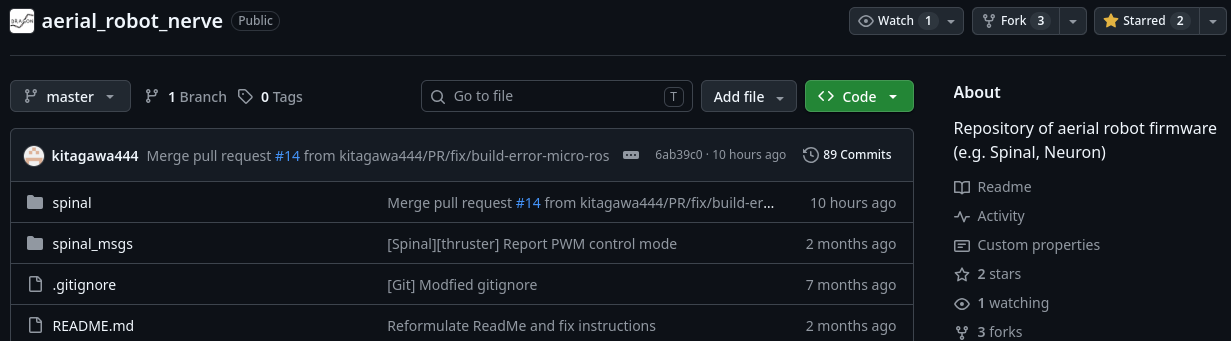
\includegraphics[width=\linewidth]{Screenshot-2026-08-28_12-23-55.png}}
  \end{cookiecard}
\end{frame}

\section{References}
\begin{frame}{Disclaimer \& Acknowledgments}
  \begin{columns}[T,onlytextwidth]
    \column{.52\textwidth}
      \cookiekicker{Author's Responsibility}
      \vspace{.5em}
      
      I take full responsibility for the content, opinions, and technical claims presented in this talk. All scientific perspectives are my own.

    \column{.45\textwidth}
      \begin{cookiecard}[title=AI Assistance Note]
        \small
        Generative AI tools were used to assist in the preparation of this presentation:
        \vspace{0.4em}
        \begin{itemize}
          \item Pre-formatting the Beamer slides.
          \item Textual review and translation.
          \item Generation of the TikZ flowchart.
        \end{itemize}
      \end{cookiecard}
  \end{columns}
\end{frame}

\begin{frame}[allowframebreaks]{References}
  \scriptsize
  \begin{thebibliography}{99}
  
    \bibitem{berlin_decl}
    Max Planck Society (2003).
    \newblock \textit{Berlin Declaration on Open Access to Knowledge in the Sciences and Humanities}.
    \newblock \url{https://openaccess.mpg.de/Berlin-Declaration}

    \bibitem{coursera_bp}
    Coursera \& University of São Paulo.
    \newblock \textit{Boas Práticas Científicas} (Good Scientific Practices Course).
    \newblock \url{https://www.coursera.org/learn/boas-praticas-cientificas}

    \bibitem{fapesp_os}
    FAPESP.
    \newblock \textit{FAPESP Open Science}.
    \newblock \url{https://www.fapesp.br/openscience/}

    \bibitem{mdpi_decl}
    MDPI Blog (2026).
    \newblock \textit{4 Defining Declarations in the History of Open Access}.
    \newblock \url{https://blog.mdpi.com/2026/08/04/4-defining-declarations-in-the-history-of-open-access/}

    \bibitem{nasm_os}
    National Academies of Sciences, Engineering, and Medicine (2018).
    \newblock \textit{Open Science by Design: Realizing a Vision for 21st Century Research}.
    \newblock Washington, DC: The National Academies Press. \url{https://doi.org/10.17226/25116}

    \bibitem{lgpd}
    Presidência da República, Brazil (2018).
    \newblock \textit{Lei nº 13.709: Lei Geral de Proteção de Dados Pessoais (LGPD)}.
    \newblock \url{https://www.planalto.gov.br/ccivil_03/_ato2015-2018/2018/lei/l13709.htm}
    
    \bibitem{fapespcapes}
    Revista Pesquisa FAPESP.
    \newblock \textit{CAPES amplia acordos com editoras e autores brasileiros poderão publicar sem custo}.
    \newblock \url{https://revistapesquisa.fapesp.br/capes-amplia-acordos-com-editoras-e-autores-brasileiros-poderao-publicar-sem-custo-em-milhares-de-periodicos/}

    \bibitem{sagan_demon}
    Sagan, Carl (2006).
    \newblock \textit{O mundo assombrado pelos demônios: a ciência vista como uma vela no escuro}.
    \newblock São Paulo: Companhia de Bolso. ISBN 978-85-359-0834-3.

    \bibitem{scielo_oa}
    SciELO in Perspective (2013).
    \newblock \textit{Evolução do Acesso Aberto: breve histórico}.
    \newblock \url{https://blog.scielo.org/blog/2013/10/21/evolucao-do-acesso-aberto-breve-historico/}

    \bibitem{cienciaecultura}
    Sociedade Brasileira para o Progresso da Ciência (SBPC) (2025).
    \newblock \textit{Ciência Aberta: O caminho para a democratização do conhecimento e a inovação colaborativa}.
    \newblock Ciência \& Cultura, 77(1). \url{http://hdl.handle.net/20.500.11832/10009}
    
    \bibitem{society_rse}
    Society of Research Software Engineering.
    \newblock \textit{Society of RSE Official Website}.
    \newblock \url{https://society-rse.org/}

    \bibitem{youtube_rse}
    TaxonWorks (2025).
    \newblock \textit{What's a Research Software Engineer (RSE)?} [Video]. YouTube.
    \newblock \url{https://youtu.be/PQuSBQSjlBc}

    \bibitem{unesco_oa}
    UNESCO.
    \newblock \textit{Open Access to Scientific Information}.
    \newblock \url{https://www.unesco.org/en/open-access}

    \bibitem{redu}
    UNICAMP.
    \newblock \textit{REDU - Repositório de Dados de Pesquisa da Unicamp}.
    \newblock \url{https://redu.unicamp.br/}

    \bibitem{usp_os}
    Universidade de São Paulo.
    \newblock \textit{Declaração USP de Apoio à Ciência Aberta}.
    \newblock \url{https://cienciaaberta.usp.br/declaracao-usp-de-apoio-a-ciencia-aberta/}

    \bibitem{aerialrobotnerve}
    UT Dragon Lab. \textit{Aerial Robot Nerve (Source Code Repository)}.
    \newblock \url{https://github.com/ut-dragon-lab/aerial_robot_nerve}

    \bibitem{fair_principles}
    Wilkinson, M., Dumontier, M., Aalbersberg, I. et al. (2016).
    \newblock \textit{The FAIR Guiding Principles for scientific data management and stewardship}.
    \newblock Sci Data 3, 160018. \url{https://doi.org/10.1038/sdata.2016.18}
  \end{thebibliography}
\end{frame}

\end{document}